\section{Evaluation of WebRTC}

\thispagestyle{empty}

In this chapter we will study how WebRTC performs in different use cases and topologies previously studied in chapter~\ref{sec:topologies}. All tests will be done using a real working environment with the tools previously mentioned in chapter~\ref{sec:testingEnv}.

\subsection{Testing devices}

For the testing of WebRTC we have used multiple devices and browsers. Since we are testing the real performance of a call the usage of some automated benchmark scripts and modules have been discarded.

One Mac carrying 2.53 GHz Intel Core i5 with Mac OS X 10.7.5 and 8 GB of RAM is used to run Chrome Canary in its latest available version. 

Fujitsu laptop with 2.13 GHz Intel Core i3 with Ubuntu 12.04 64-bit and 4 GB of RAM will be running Chrome Unstable to its latest version. Both of them carrying built-in cameras and microphone.

From the browser perspective we will be using Chrome Canary, when available, or Chrome Unstable/Beta for Ubuntu.

\subsection{Point-to-point}

In a point-to-point scenario we have performed different tests to calculate how the application performs. 

Firstly we have stablished a simple call between two peers that handle video and audio in an open WiFi network. This network does not carry any UDP packet filter or FW, the connection is performed without the need of STUN or TURN, we could easily say it straight forward peer-to-peer connection. The aim of this test is to observe how the captures differ between origin and receiver on the {\it StatsAPI} and {\it ConMon} layer.

 \begin{figure}[h]
  \centering
    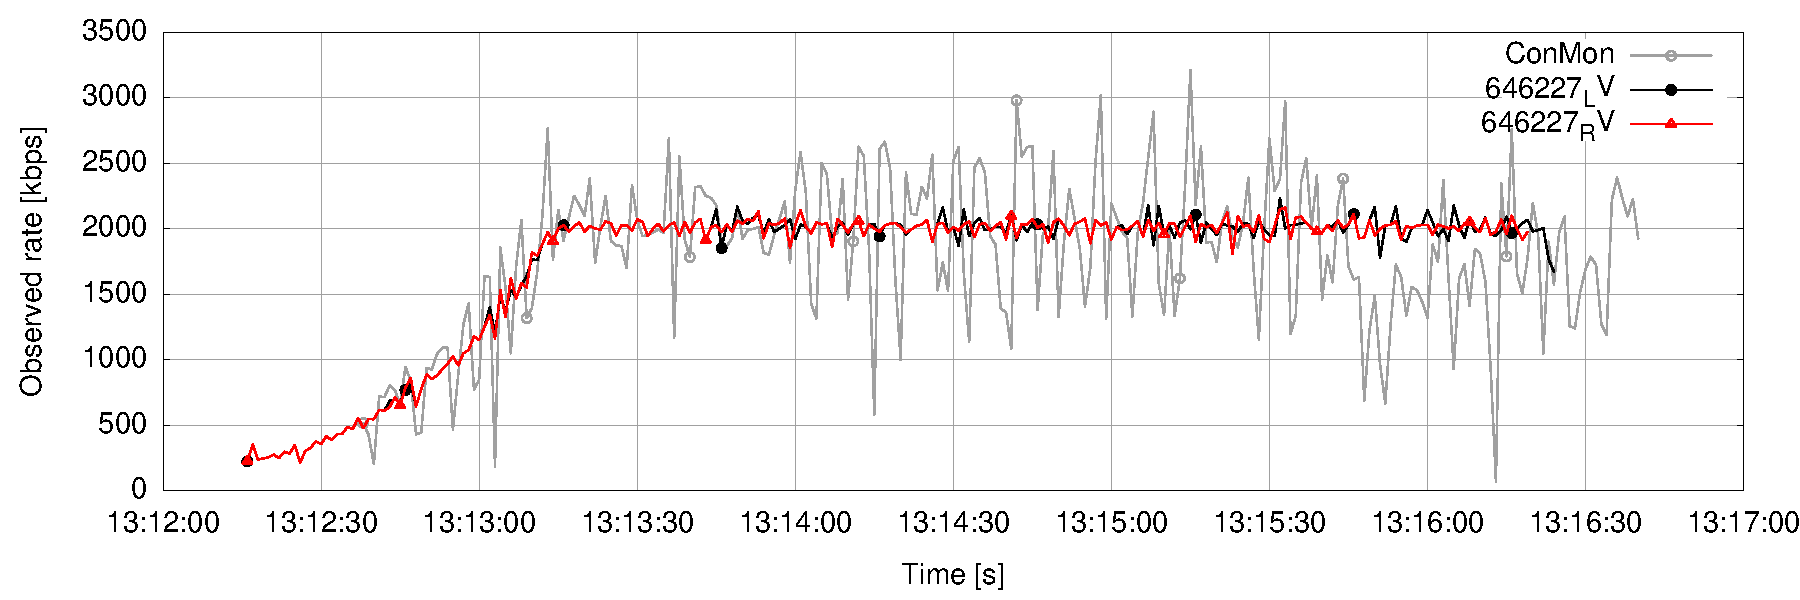
\includegraphics[width=1\textwidth]{./figures/onetoone_wifi_statsconmon.pdf}
      \caption[Point-to-point video stream plot using StatsAPI and ConMon data over WiFi]{Point-to-point video stream plot using StatsAPI and ConMon data over WiFi.}
	\label{fig:onetooneWifistatsconmon}
\end{figure}

Figure~\ref{fig:onetooneWifistatsconmon} represents the throughput rate on the same video stream, the three lines are the comparison between local video stream in origin peer, remote video stream in receiver peer and {\it ConMon} capture of the remote video stream on the receiver peer. All three streams contain the same data but they are measured in different layers, this will help us to understand the difference of throughput that is handling the overhead of the RTP and the disruption caused by the WiFi network.

Notice that red and black colors represent the Local Video (LV) and Remote Video (RV) from the same SSRC, both captures indicate the same stream captured using {\it StatsAPI}, and the grey line plots the capture performed using {\it ConMon} of the same SSRC. It is easy to observe that both {\it StatsAPI} captures are similar, some offset is produced due to the processing time between the network layer and the browser API that returns all values. Besides this, the capture is neat and throughput at the output of the origin client and input of the receiver is similar. Capture in the network layer is more abrupt as all packets are captured and the period of calculus when plotting affects when the value is added, when having two opposite values peaks they should be balanced, meaning that the transmission in most of the period is stable and the peaks when plotting are a result of accuracy. Call duration in this test has been around five minutes. Some areas, mostly between 13.15.30 and 13.16.00, show a strange behavior of the link that might be produced by the WiFi, this throughput distortion is balanced on the WebRTC layer as the throughput delivered by the API does not change.

When we try to measure the quality of the call one important indicator is the delay, to calculate the delay we can either use the RTT measured by our {\it StatsAPI} or use the captures performed on the network layer by {\it ConMon}. The {\it ConMon} procedure will give us a high accuracy on the delay subtracting both timestamps from both of the clients, this will require to calculate the drift of the internal clock of the computers and balance the deviation.

 \begin{figure}[h]
  \centering
    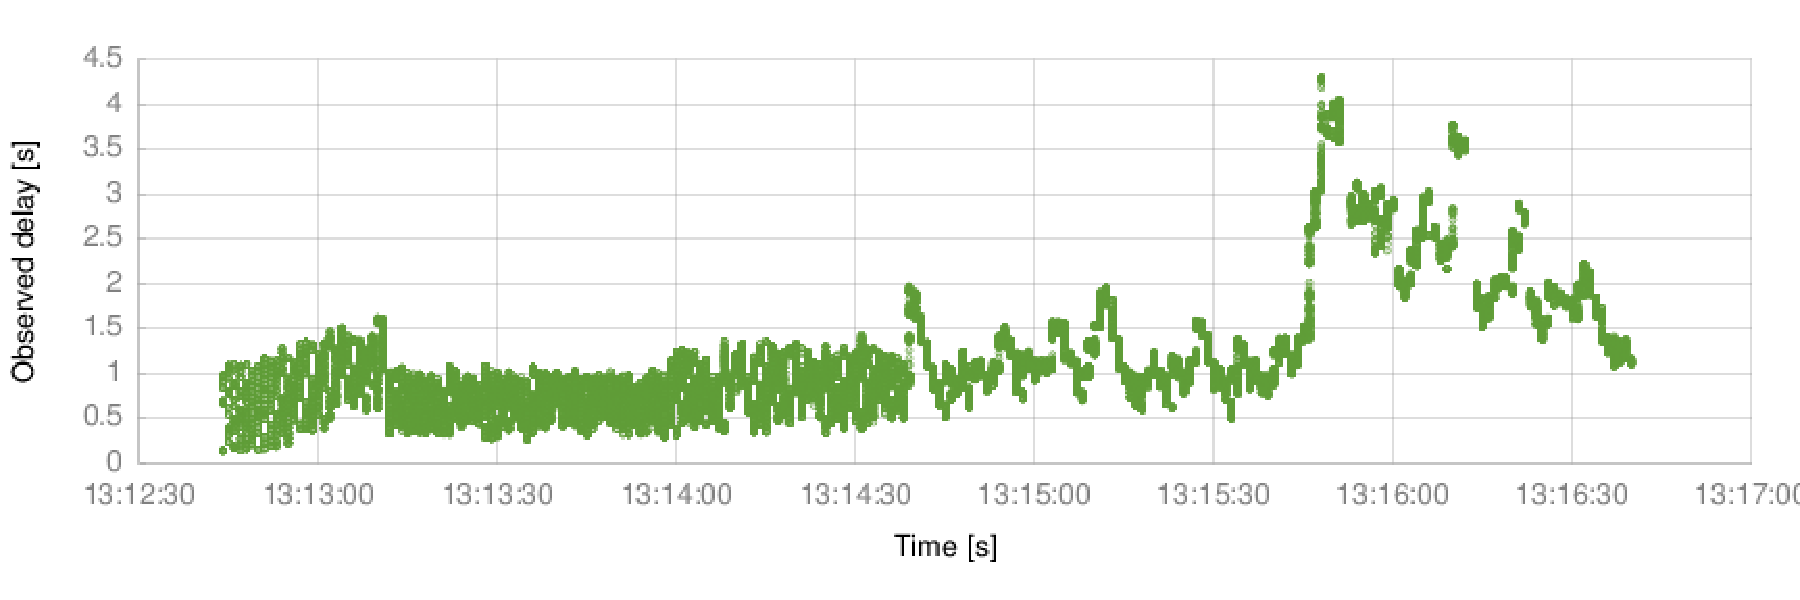
\includegraphics[width=1\textwidth]{./figures/delay_116_646227.pdf}
      \caption[Delay calculated on the same stream captured using ConMon in both ends over WiFi]{Delay calculated on the same stream captured using ConMon in both ends over WiFi.}
	\label{fig:delay_116_646227}
\end{figure}

Figure~\ref{fig:delay_116_646227} represents the delay of the stream plotted in~\ref{fig:onetooneWifistatsconmon}. We can see that the quality of the call is affected by the network distortion at the end of Figure~\ref{fig:onetooneWifistatsconmon}, this variation of the throughput delivers a high delay of more than 4 seconds during some period of time between 13:15:30 and 13:16:30, the media received at that time will not render correctly and the user experience of the call is going to be worst than at the beginning of the establishment.

